% !TEX root = main.tex

\section{事务} % Chap 14
\begin{definition}[事务(transaction)]
构成单一逻辑工作单元的操作集合称为事务。
即使有故障,数据库系统也必须保证数据库的正确执行——要么执行整个事务,要么属于该事务的操作一个也不执行。
\end{definition}

事务具有以下的基本性质:
\begin{itemize}
	\item 原子性:要么执行完,要么不执行,不能执行到一半。
	\item 一致性:除了基本的数据完整性约束,还有更多的一致性约束。
	\item 隔离性:每个事务都察觉不到系统中有其他事务在并发执行,一定是完成一个再进行下一个。
	\item 持久性:一个事务成功完成对数据库的改变是永久的,即使出现系统故障。
\end{itemize}

事务的基本状态:
\begin{itemize}
	\item 活动的(active):初始状态
	\item 部分提交的(partially commited):最后一条语句执行后
	\item 失败的(failed):执行出错
	\item 中止的(aborted):事务回滚且数据库已恢复到事务开始执行前
	\item 提交的(commited):成功完成
\end{itemize}
\begin{figure}[H]
\centering
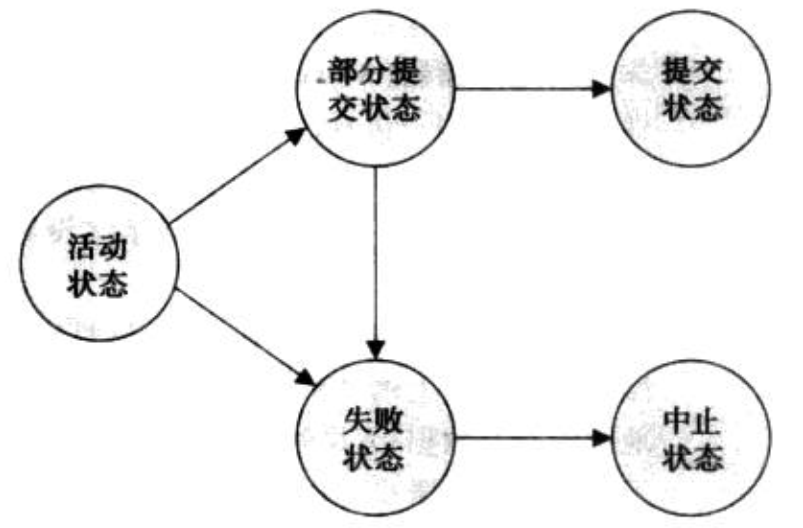
\includegraphics[width=0.5\linewidth]{fig/transaction_state.png}
\end{figure}

\begin{definition}[冲突]
当$I$和$J$是不同事务在相同数据项上的操作,并且其中至少有一个是\verb'write'指令时,则称$I$与$J$是冲突的。
\end{definition}
\begin{definition}[冲突等价(conflict equivalent)]
如果调度$S$可以经过一系列非冲突指令交换转换为$S'$,则称$S$和$S'$是冲突等价的。
若$S'$为串行调度,则$S$为冲突可串行化的(conflict serializable)。
\end{definition}

可以通过构造一个优先图(precedence graph)来判断是否冲突可串行化。
如果无环(用环检测算法),则冲突可串行化,可以通过拓扑排序得到串行化顺序。

隔离性级别:
\begin{itemize}
	\item 可串行化(serializable)
	\item 可重复读(repeatable read)
	\item 已提交读(read committed)
	\item 未提交读(read uncommitted)
\end{itemize}

隔离性级别的实现:并发控制机制
\begin{itemize}
	\item 锁
	\item 时间戳:读时间戳记录读该数据项的事务的最大/最近时间戳,写时间戳记录写入该数据项当前值的事务的时间戳。
	时间戳用来确保在访问冲突情况下,事务按照事务时间戳顺序来访问数据项。
	当不可能访问时,违例事务会中止,并且分配一个新的时间戳重新开始
	\item 多版本与快照隔离(snapshot isolation)
\end{itemize}